\newpage
\section{TGGs in action}
\genHeader
\label{sect:TGGs_in_Action}

In order to perform a forwards or backwards transformation, we need to actually create something for the TGG to work with. In other words, we need to create an
instance model\footnote{For a detailed review, refer to Part II, Section 3} of either our target or our source metamodel! Since dictionaries are a much simpler
structure, let's start with the backwards transformation, from \texttt{DictionaryToBox}.

\begin{itemize}

\item[$\blacktriangleright$] Navigate to \texttt{Dictionary\-Language/model/} and open \texttt{Dictio\-nary\-Lang\-uage.ecore}. Create a new
dynamic instance of a \texttt{Dictionary} named \texttt{target.xmi}. Don't quickly press \texttt{enter}! Make sure you persist it in
\texttt{Learn\-ing\-Box\-To\-Dictionary\-In\-te\-gra\-tion/in\-stan\-ces/} (Fig.~\ref{fig:create_instance_dict}).

\begin{figure}[htbp]
\begin{center}
  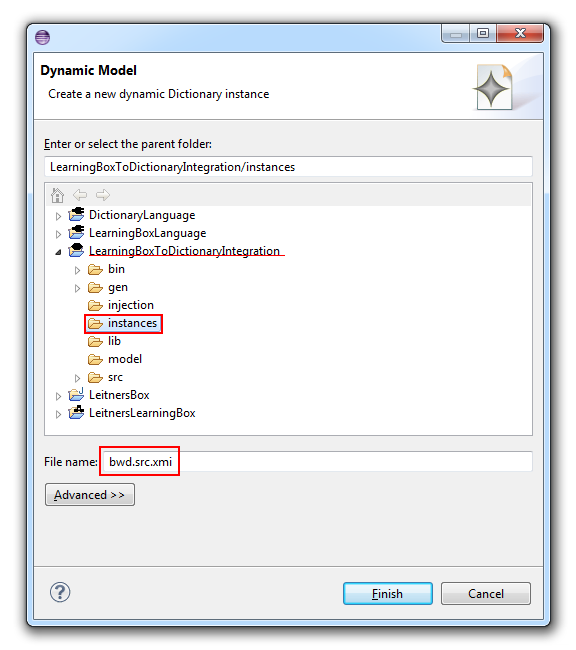
\includegraphics[width=0.8\textwidth]{eclipse_dictionaryInstance}
  \caption{Create a dynamic instance of \texttt{Dictionary}}
  \label{fig:create_instance_dict}
\end{center}
\end{figure}

\newpage

\item[$\blacktriangleright$] Open \texttt{target.xmi}, and edit the \texttt{Dictionary} properties by setting \texttt{Title} to \texttt{English Numbers}. This
will be manipulated by the constraint to become \texttt{box.name}.

\item[$\blacktriangleright$] Create three child \texttt{Entry} objects, giving each one a different difficulty level. Remember, the content follows a specific
syntax based on the concatnation constraint we created in the \texttt{CardToEntryRule}:
\syntax{word : meaning}
Your target instance should come to resemble Fig.~\ref{fig:dictionaryxmi}

\begin{figure}[htbp]
\begin{center}
  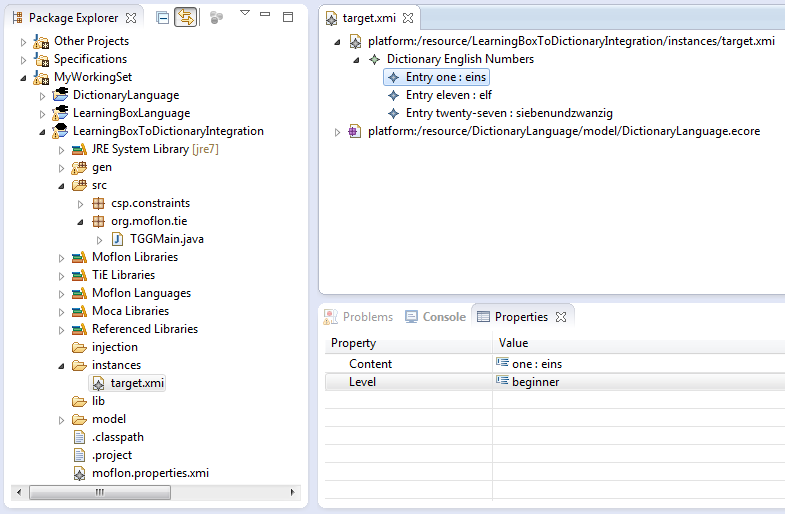
\includegraphics[width=\textwidth]{eclipse_addEntries}
  \caption{Contents of the dictionary}
  \label{fig:dictionaryxmi}
\end{center}
\end{figure}

\item[$\blacktriangleright$] Navigate to ``LearningBox\-To\-Dictionary\-In\-te\-gra\-tion\-/src'' and right-click on \texttt{TGGMain.java}. Go to ``Run
as\ldots/Java Application''

\item[$\blacktriangleright$] Did you get one error message, followed by one success message eMoflon console below the editor? Perfect! That's exactly what we
expected (Fig.~\ref{fig:tggERROR}). Both of these statements make sense -- our TGG first attempted a forward transformation of \texttt{box} to
\texttt{dictionary} but, given that it was missing the source (\texttt{box}) instance, it was only able to perform a transformation in the backwards direction.

\begin{figure}[htbp]
\begin{center}
  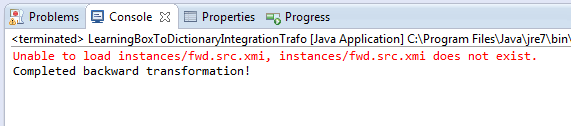
\includegraphics[width=\textwidth]{eclipse_TGGError}
  \caption{comment}
  \label{fig:tggERROR}
\end{center}
\end{figure}

\newpage

\item[$\blacktriangleright$] Refresh the integration's \texttt{instances} folder. There should now be four new \texttt{xmi} files. While you created
\texttt{target}, the TGG created \texttt{corr\_BWD}, correspondence graph between target and source, \texttt{protocol\_BWD}, a listing of the attempted
and successful steps taken in the backwards transformation, and \texttt{target.xmi\_BWD}, the result of the transformation. Open this file in the editor.

\item[$\blacktriangleright$] Its an \texttt{English Numbers Box!} Expand the tree and you'll see our \texttt{Dictionary} now translated backward into
a box containing three \texttt{Par\-ti\-tions}, as specified in \texttt{Box\-To\-Dictionary\-Rule} (Fig.~\ref{fig:derivedBOX}). Those partitions are then filled
according to their \texttt{index} and the \texttt{entry}'s difficulty, as specified in the \texttt{IndexToLevelConstraint} in \texttt{CardToEntry}. If you
double click on each \texttt{card} to view its properties, you can see the \texttt{back} and \texttt{face} have also been satisfied accordingly.

\begin{figure}[htbp]
\begin{center}
  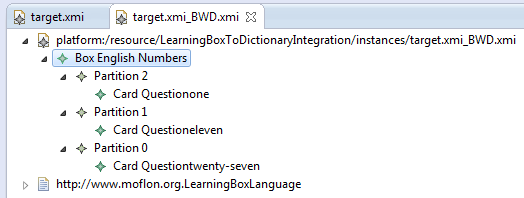
\includegraphics[width=\textwidth]{eclipse_TGGRuleBuiltBOX}
  \caption{our created box}
  \label{fig:derivedBOX}
\end{center}
\end{figure}

\clearpage

\item[$\blacktriangleright$] Don't forget about one of eMoflon neat visualizing features - the graph viewer! This is an especially useful tool with TGGs when
you need to do a quick confirmation that your transformation was successful. To practice, drag-and-drop \texttt{Box English Numbers} into the window. You can
see the \texttt{partition}s properly connected via link variables, and you can see each \texttt{card} in its proper place (Fig.~\ref{fig:graphViewBox}). You
could also try viewing the source \texttt{Dictionary} this way as well, but unfortunately you'll only have a terribly uninteresting simple tree graph, with
three long lines connecting each entry to the dictionary.

\begin{figure}[htbp]
\begin{center}
  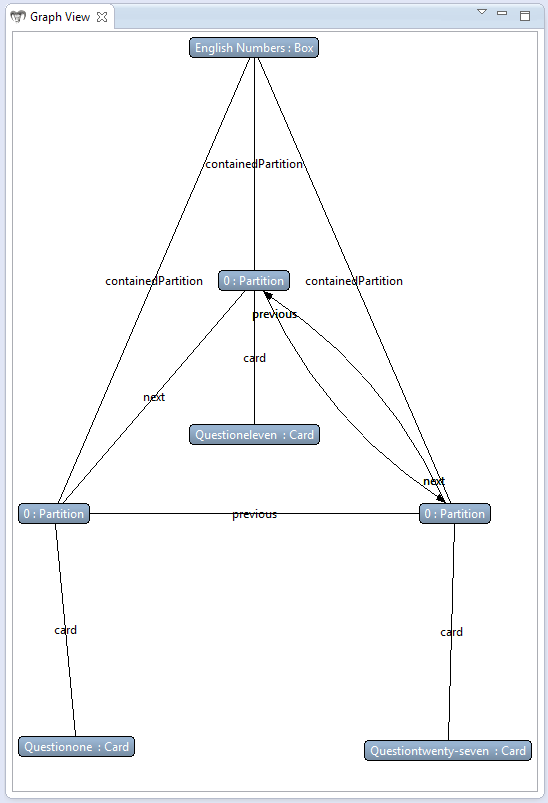
\includegraphics[width=0.8\textwidth]{eclipse_EngNumBoxGraphView}
  \caption{dat graph view. hmmmm.}
  \label{fig:graphViewBox}
\end{center}
\end{figure}


\vspace{0.5cm}

Congratulations! You have successfully performed your first \emph{backward} transformation from your target model (dictionary) to your source (Learning box)
using TGGs! To show that the transformation is actually bidirectional however, lets edit the source model (thus resolving the error), and run the TGG again to
transform \texttt{box} forward into a \texttt{Dictionary}.


\item[$\blacktriangleright$] Make a copy of \texttt{target.xmi\_BWD.xmi} (the result of the backward transformation)
and rename it to \texttt{source.xmi}.
  
% \item[$\blacktriangleright$] Open \texttt{source.xmi} and create some new \texttt{Card} objects in the \texttt{Partition}s (e.g., create a new \texttt{Card}
% with \texttt{Card.face = ``Question : two''}, \texttt{Card.back = ``Answer : zwei''} in \texttt{Partition 0}).

\item[$\blacktriangleright$] Run the \texttt{TGGMain.java} again by pressing the green ``Run As\ldots'' icon on the toolbar. You should now have two success
messages in the console window! Inspect \texttt{source.xmi\_FWD.xmi}, the result of the forward transformation, and the original target model. If everything was
created and executed properly, they should look exactly the same! Great work!

\end{itemize}
